\chapter{細節實現題}
這類題目不考特定的算法,純粹考察寫代碼的熟練度。
\newline


\section{Reverse Integer} %%%%%%%%%%%%%%%%%%%%%%%%%%%%%%
\label{sec:reverse-integer}


\subsubsection{描述}
Reverse digits of an integer.

Example1: x = 123, return 321

Example2: x = -123, return -321


\textbf{Have you thought about this?}

Here are some good questions to ask before coding. Bonus points for you if you have already thought through this!

If the integer's last digit is 0, what should the output be? ie, cases such as 10, 100.

Did you notice that the reversed integer might overflow? Assume the input is a 32-bit integer, then the reverse of 1000000003 overflows. How should you handle such cases?

Throw an exception? Good, but what if throwing an exception is not an option? You would then have to re-design the function (ie, add an extra parameter).


\subsubsection{分析}
短小精悍的題,代碼也可以寫的很短小。


\subsubsection{代碼}
\begin{Code}
//LeetCode, Reverse Integer
// 時間複雜度O(logn),空間複雜度O(1)
// 考慮 1.負數的情況 2. 溢出的情況(正溢出&&負溢出,比如 x = -2147483648(即-2^31) )
class Solution {
public:
    int reverse (int x) {
        long long r = 0;
        long long t = x;
        t = t > 0 ? t : -t;
        for (; t; t /= 10)
            r = r * 10 + t % 10;

        bool sign = x > 0 ? false: true;
        if (r > 2147483647 || (sign && r > 2147483648)) {
            return 0;
        } else {
            if (sign) {
                return -r;
            } else {
                return r;
            }
        }
    }
};
\end{Code}


\subsubsection{相關題目}
\begindot
\item Palindrome Number, 見 \S \ref{sec:palindrome-number}
\myenddot


\section{Palindrome Number} %%%%%%%%%%%%%%%%%%%%%%%%%%%%%%
\label{sec:palindrome-number}


\subsubsection{描述}
Determine whether an integer is a palindrome. Do this without extra space.

\textbf{Some hints:}

Could negative integers be palindromes? (ie, -1)

If you are thinking of converting the integer to string, note the restriction of using extra space.

You could also try reversing an integer. However, if you have solved the problem "Reverse Integer", you know that the reversed integer might overflow. How would you handle such case?

There is a more generic way of solving this problem.


\subsubsection{分析}
首先想到,可以利用上一題,將整數反轉,然後與原來的整數比較,是否相等,相等則為 Palindrome 的。可是 reverse()會溢出。

正確的解法是,不斷地取第一位和最後一位(10進制下)進行比較,相等則取第二位和倒數第二位,直到完成比較或者中途找到了不一致的位。


\subsubsection{代碼}
\begin{Code}
//LeetCode, Palindrome Number
// 時間複雜度O(1),空間複雜度O(1)
class Solution {
public:
    bool isPalindrome(int x) {
        if (x < 0) return false;
        int d = 1; // divisor
        while (x / d >= 10) d *= 10;

        while (x > 0) {
            int q = x / d;  // quotient
            int r = x % 10;   // remainder
            if (q != r) return false;
            x = x % d / 10;
            d /= 100;
        }
        return true;
    }
};
\end{Code}


\subsubsection{相關題目}
\begindot
\item Reverse Integer, 見 \S \ref{sec:reverse-integer}
\item Valid Palindrome, 見 \S \ref{sec:valid-palindrome}
\myenddot


\section{Insert Interval} %%%%%%%%%%%%%%%%%%%%%%%%%%%%%%
\label{sec:insert-interval}


\subsubsection{描述}
Given a set of non-overlapping intervals, insert a new interval into the intervals (merge if necessary).

You may assume that the intervals were initially sorted according to their start times.

Example 1:
Given intervals \code\{[1,3],[6,9]\}, insert and merge \code\{[2,5]\} in as \code\{[1,5],[6,9]\}.

Example 2:
Given \code\{[1,2],[3,5],[6,7],[8,10],[12,16]\}, insert and merge \code\{[4,9]\} in as \code\{[1,2],[3,10],[12,16]\}.

This is because the new interval \code\{[4,9]\} overlaps with \code\{[3,5],[6,7],[8,10]\}.


\subsubsection{分析}
無


\subsubsection{代碼}
\begin{Code}
struct Interval {
    int start;
    int end;
    Interval() : start(0), end(0) { }
    Interval(int s, int e) : start(s), end(e) { }
};

//LeetCode, Insert Interval
// 時間複雜度O(n),空間複雜度O(1)
class Solution {
public:
    vector<Interval> insert(vector<Interval> &intervals, Interval newInterval) {
        vector<Interval>::iterator it = intervals.begin();
        while (it != intervals.end()) {
            if (newInterval.end < it->start) {
                intervals.insert(it, newInterval);
                return intervals;
            } else if (newInterval.start > it->end) {
                it++;
                continue;
            } else {
                newInterval.start = min(newInterval.start, it->start);
                newInterval.end = max(newInterval.end, it->end);
                it = intervals.erase(it);
            }
        }
        intervals.insert(intervals.end(), newInterval);
        return intervals;
    }
};
\end{Code}


\subsubsection{相關題目}

\begindot
\item Merge Intervals,見 \S \ref{sec:merge-intervals}
\myenddot


\section{Merge Intervals} %%%%%%%%%%%%%%%%%%%%%%%%%%%%%%
\label{sec:merge-intervals}


\subsubsection{描述}
Given a collection of intervals, merge all overlapping intervals.

For example,
Given \code\{[1,3],[2,6],[8,10],[15,18]\},
return \code\{[1,6],[8,10],[15,18]\}


\subsubsection{分析}
複用一下Insert Intervals的解法即可,創建一個新的interval集合,然後每次從舊的裏面取一個interval出來,然後插入到新的集合中。


\subsubsection{代碼}
\begin{Code}
struct Interval {
    int start;
    int end;
    Interval() : start(0), end(0) { }
    Interval(int s, int e) : start(s), end(e) { }
};

//LeetCode, Merge Interval
//複用一下Insert Intervals的解法即可
// 時間複雜度O(n1+n2+...),空間複雜度O(1)
class Solution {
public:
    vector<Interval> merge(vector<Interval> &intervals) {
        vector<Interval> result;
        for (int i = 0; i < intervals.size(); i++) {
            insert(result, intervals[i]);
        }
        return result;
    }
private:
    vector<Interval> insert(vector<Interval> &intervals, Interval newInterval) {
        vector<Interval>::iterator it = intervals.begin();
        while (it != intervals.end()) {
            if (newInterval.end < it->start) {
                intervals.insert(it, newInterval);
                return intervals;
            } else if (newInterval.start > it->end) {
                it++;
                continue;
            } else {
                newInterval.start = min(newInterval.start, it->start);
                newInterval.end = max(newInterval.end, it->end);
                it = intervals.erase(it);
            }
        }
        intervals.insert(intervals.end(), newInterval);
        return intervals;
    }
};
\end{Code}
\subsubsection{代碼}
\begin{Code}
//LeetCode, Merge Interval
// Sort it and always push back into a reserved vector
// 時間複雜度O(nlogn),空間複雜度O(n)
class Solution {
public:
    vector<vector<int>> merge(vector<vector<int>>& intervals) {
        // sort it first
        sort(intervals.begin(), intervals.end(), [&](const auto& first, const auto& second)
             {
                return first[0] < second[0];
             });
        vector<vector<int>> result;
        result.reserve(intervals.size());

        for (const auto& interval : intervals)
            mergeBack(result, interval);

        return result;
    }
private:
    void mergeBack(vector<vector<int>>& result, const vector<int>& interval) {
        if (result.size() == 0) result.push_back(interval);

        int& start = result.back()[0];
        int& end = result.back()[1];

        if (interval[0] >= start && interval[0] <= end)
            end = max(end, interval[1]);
        else
            result.push_back(interval);
    }
};
\end{Code}


\subsubsection{相關題目}

\begindot
\item Insert Interval,見 \S \ref{sec:insert-interval}
\myenddot


\section{Minimum Window Substring} %%%%%%%%%%%%%%%%%%%%%%%%%%%%%%
\label{sec:minimum-window-substring}


\subsubsection{描述}
Given a string $S$ and a string $T$, find the minimum window in $S$ which will contain all the characters in $T$ in complexity $O(n)$.

For example, \code{S = "ADOBECODEBANC", T = "ABC"}

Minimum window is \code{"BANC"}.

Note:
\begindot
\item If there is no such window in $S$ that covers all characters in $T$, return the emtpy string \code{""}.
\item If there are multiple such windows, you are guaranteed that there will always be only one unique minimum window in $S$.
\myenddot


\subsubsection{分析}
雙指針,動態維護一個區間。尾指針不斷往後掃,當掃到有一個窗口包含了所有$T$的字符後,然後再收縮頭指針,直到不能再收縮為止。最後記錄所有可能的情況中窗口最小的


\subsubsection{代碼}
\begin{Code}
// LeetCode, Minimum Window Substring
// 時間複雜度O(n),空間複雜度O(1)
class Solution {
public:
    string minWindow(string S, string T) {
        if (S.empty()) return "";
        if (S.size() < T.size()) return "";

        const int ASCII_MAX = 256;
        int appeared_count[ASCII_MAX];
        int expected_count[ASCII_MAX];
        fill(appeared_count, appeared_count + ASCII_MAX, 0);
        fill(expected_count, expected_count + ASCII_MAX, 0);

        for (size_t i = 0; i < T.size(); i++) expected_count[T[i]]++;

        int minWidth = INT_MAX, min_start = 0;  // 窗口大小,起點
        int wnd_start = 0;
        int appeared = 0;  // 完整包含了一個T
        //尾指針不斷往後掃
        for (size_t wnd_end = 0; wnd_end < S.size(); wnd_end++) {
            if (expected_count[S[wnd_end]] > 0)  {  // this char is a part of T
                appeared_count[S[wnd_end]]++;
                if (appeared_count[S[wnd_end]] <= expected_count[S[wnd_end]])
                    appeared++;
            }
            if (appeared == T.size()) {  // 完整包含了一個T
                // 收縮頭指針
                while (appeared_count[S[wnd_start]] > expected_count[S[wnd_start]]
                        || expected_count[S[wnd_start]] == 0) {
                    appeared_count[S[wnd_start]]--;
                    wnd_start++;
                }
                if (minWidth > (wnd_end - wnd_start + 1)) {
                    minWidth = wnd_end - wnd_start + 1;
                    min_start = wnd_start;
                }
            }
        }

        if (minWidth == INT_MAX) return "";
        else return S.substr(min_start, minWidth);
    }
};
\end{Code}


\subsubsection{相關題目}

\begindot
\item 無
\myenddot


\section{Multiply Strings} %%%%%%%%%%%%%%%%%%%%%%%%%%%%%%
\label{sec:multiply-strings}


\subsubsection{描述}
Given two numbers represented as strings, return multiplication of the numbers as a string.

Note: The numbers can be arbitrarily large and are non-negative.


\subsubsection{分析}
高精度乘法。

常見的做法是將字符轉化為一個int,一一對應,形成一個int數組。但是這樣很浪費空間,一個int32的最大值是$2^{31}-1=2147483647$,可以與9個字符對應,由於有乘法,減半,則至少可以與4個字符一一對應。一個int64可以與9個字符對應。


\subsubsection{代碼1}
\begin{Code}
// LeetCode, Multiply Strings
// @author 連城 (http://weibo.com/lianchengzju)
// 一個字符對應一個int
// 時間複雜度O(n*m),空間複雜度O(n+m)
typedef vector<int> bigint;

bigint make_bigint(string const& repr) {
    bigint n;
    transform(repr.rbegin(), repr.rend(), back_inserter(n),
            [](char c) { return c - '0'; });
    return n;
}

string to_string(bigint const& n) {
    string str;
    transform(find_if(n.rbegin(), prev(n.rend()),
            [](char c) { return c > '\0'; }), n.rend(), back_inserter(str),
            [](char c) { return c + '0'; });
    return str;
}

bigint operator*(bigint const& x, bigint const& y) {
    bigint z(x.size() + y.size());

    for (size_t i = 0; i < x.size(); ++i)
        for (size_t j = 0; j < y.size(); ++j) {
            z[i + j] += x[i] * y[j];
            z[i + j + 1] += z[i + j] / 10;
            z[i + j] %= 10;
        }

    return z;
}

class Solution {
public:
    string multiply(string num1, string num2) {
        return to_string(make_bigint(num1) * make_bigint(num2));
    }
};
\end{Code}


\subsubsection{代碼2}
\begin{Code}
// LeetCode, Multiply Strings
// 9個字符對應一個int64_t
// 時間複雜度O(n*m/81),空間複雜度O((n+m)/9)
/** 大整數類. */
class BigInt {
public:
    /**
     * @brief 構造函數,將字符串轉化為大整數.
     * @param[in] s 輸入的字符串
     * @return 無
     */
    BigInt(string s) {
        vector<int64_t> result;
        result.reserve(s.size() / RADIX_LEN + 1);

        for (int i = s.size(); i > 0; i -= RADIX_LEN) {  // [i-RADIX_LEN, i)
            int temp = 0;
            const int low = max(i - RADIX_LEN, 0);
            for (int j = low; j < i; j++) {
                temp = temp * 10 + s[j] - '0';
            }
            result.push_back(temp);
        }
        elems = result;
    }
    /**
     * @brief 將整數轉化為字符串.
     * @return 字符串
     */
    string toString() {
        stringstream result;
        bool started = false; // 用於跳過前導0
        for (auto i = elems.rbegin(); i != elems.rend(); i++) {
            if (started) { // 如果多餘的0已經都跳過,則輸出
                result << setw(RADIX_LEN) << setfill('0') << *i;
            } else {
                result << *i;
                started = true; // 碰到第一個非0的值,就説明多餘的0已經都跳過
            }
        }

        if (!started) return "0"; // 當x全為0時
        else return result.str();
    }

    /**
     * @brief 大整數乘法.
     * @param[in] x x
     * @param[in] y y
     * @return 大整數
     */
    static BigInt multiply(const BigInt &x, const BigInt &y) {
        vector<int64_t> z(x.elems.size() + y.elems.size(), 0);

        for (size_t i = 0; i < y.elems.size(); i++) {
            for (size_t j = 0; j < x.elems.size(); j++) { // 用y[i]去乘以x的各位
                //  兩數第i, j位相乘,累加到結果的第i+j位
                z[i + j] += y.elems[i] * x.elems[j];

                if (z[i + j] >= BIGINT_RADIX) { //  看是否要進位
                    z[i + j + 1] += z[i + j] / BIGINT_RADIX; //  進位
                    z[i + j] %= BIGINT_RADIX;
                }
            }
        }
        while (z.back() == 0) z.pop_back();  // 沒有進位,去掉最高位的0
        return BigInt(z);
    }

private:
    typedef long long int64_t;
    /** 一個數組元素對應9個十進制位,即數組是億進制的
     * 因為 1000000000 * 1000000000 沒有超過 2^63-1
     */
    const static int BIGINT_RADIX = 1000000000;
    const static int RADIX_LEN = 9;
    /** 萬進制整數. */
    vector<int64_t> elems;
    BigInt(const vector<int64_t> num) : elems(num) {}
};


class Solution {
public:
    string multiply(string num1, string num2) {
        BigInt x(num1);
        BigInt y(num2);
        return BigInt::multiply(x, y).toString();
    }
};
\end{Code}


\subsubsection{相關題目}

\begindot
\item 無
\myenddot


\section{Substring with Concatenation of All Words} %%%%%%%%%%%%%%%%%%%%%%%%%%%%%%
\label{sec:substring-with-concatenation-of-all-words}


\subsubsection{描述}
You are given a string, $S$, and a list of words, $L$, that are all of the same length. Find all starting indices of substring(s) in $S$ that is a concatenation of each word in $L$ exactly once and without any intervening characters.

For example, given:
\begin{Code}
S: "barfoothefoobarman"
L: ["foo", "bar"]
\end{Code}

You should return the indices: \code\{[0,9]\}.(order does not matter).


\subsubsection{分析}
無


\subsubsection{代碼}
\begin{Code}
// LeetCode, Substring with Concatenation of All Words
// 時間複雜度O(n*m),空間複雜度O(m)
class Solution {
public:
    vector<int> findSubstring(string s, vector<string>& dict) {
        size_t wordLength = dict.front().length();
        size_t catLength = wordLength * dict.size();
        vector<int> result;

        if (s.length() < catLength) return result;

        unordered_map<string, int> wordCount;

        for (auto const& word : dict) ++wordCount[word];

        for (auto i = begin(s); i <= prev(end(s), catLength); ++i) {
            unordered_map<string, int> unused(wordCount);

            for (auto j = i; j != next(i, catLength); j += wordLength) {
                auto pos = unused.find(string(j, next(j, wordLength)));

                if (pos == unused.end() || pos->second == 0) break;

                if (--pos->second == 0) unused.erase(pos);
            }

            if (unused.size() == 0) result.push_back(distance(begin(s), i));
        }

        return result;
    }
};
\end{Code}


\subsubsection{相關題目}

\begindot
\item 無
\myenddot


\section{Pascal's Triangle} %%%%%%%%%%%%%%%%%%%%%%%%%%%%%%
\label{sec:pascal-s-triangle}


\subsubsection{描述}
Given $numRows$, generate the first $numRows$ of Pascal's triangle.

For example, given $numRows = 5$,

Return
\begin{Code}
[
     [1],
    [1,1],
   [1,2,1],
  [1,3,3,1],
 [1,4,6,4,1]
]
\end{Code}


\subsubsection{分析}
本題可以用隊列,計算下一行時,給上一行左右各加一個0,然後下一行的每個元素,就等於左上角和右上角之和。

另一種思路,下一行第一個元素和最後一個元素賦值為1,中間的每個元素,等於上一行的左上角和右上角元素之和。


\subsubsection{從左到右}
\begin{Code}
// LeetCode, Pascal's Triangle
// 時間複雜度O(n^2),空間複雜度O(n)
class Solution {
public:
    vector<vector<int> > generate(int numRows) {
        vector<vector<int> > result;
        if(numRows == 0) return result;

        result.push_back(vector<int>(1,1)); //first row

        for(int i = 2; i <= numRows; ++i) {
            vector<int> current(i,1);  // 本行
            const vector<int> &prev = result[i-2];  // 上一行

            for(int j = 1; j < i - 1; ++j) {
                current[j] = prev[j-1] + prev[j]; // 左上角和右上角之和
            }
            result.push_back(current);
        }
        return result;
    }
};
\end{Code}


\subsubsection{從右到左}
\begin{Code}
// LeetCode, Pascal's Triangle
// 時間複雜度O(n^2),空間複雜度O(n)
class Solution {
public:
    vector<vector<int> > generate(int numRows) {
        vector<vector<int> > result;
        vector<int> array;
        for (int i = 1; i <= numRows; i++) {
            for (int j = i - 2; j > 0; j--) {
                array[j] = array[j - 1] + array[j];
            }
            array.push_back(1);
            result.push_back(array);
        }
        return result;
    }
};
\end{Code}


\subsubsection{相關題目}
\begindot
\item Pascal's Triangle II,見 \S \ref{sec:pascals-triangle-ii}
\myenddot


\section{Pascal's Triangle II} %%%%%%%%%%%%%%%%%%%%%%%%%%%%%%
\label{sec:pascal-s-triangle-ii}


\subsubsection{描述}
Given an index $k$, return the $k^{th}$ row of the Pascal's triangle.

For example, given $k = 3$,

Return \code\{[1,3,3,1]\}.

Note: Could you optimize your algorithm to use only $O(k)$ extra space?


\subsubsection{分析}
滾動數組。


\subsubsection{代碼}

\begin{Code}
// LeetCode, Pascal's Triangle II
// 滾動數組,時間複雜度O(n^2),空間複雜度O(n)
class Solution {
public:
  vector<int> getRow(int rowIndex) {
    vector<int> array;
    for (int i = 0; i <= rowIndex; i++) {
      for (int j = i - 1; j > 0; j--){
        array[j] = array[j - 1] + array[j];
      }
      array.push_back(1);
    }
    return array;
  }
};
\end{Code}

\subsubsection{遞歸}
\begin{Code}
// LeetCode, Pascal's Triangle II
// 滾動數組,時間複雜度O(n^2),空間複雜度O(n)
class Solution {
public:
    vector<int> getRow(int rowIndex) {
        vector<int> result;
        getRow(result, rowIndex, 0);
        return result;
    }
private:
    void getRow(vector<int>& result, int rowIndex, int step) {
        if (step > rowIndex) return;

        for (int i = step - 1; i > 0; i--)
            result[i] = result[i-1] + result[i];
        result.push_back(1);

        getRow(result, rowIndex, step+1);
    }
};
\end{Code}

\subsubsection{相關題目}
\begindot
\item Pascal's Triangle,見 \S \ref{sec:pascal-s-triangle}
\myenddot


\section{Spiral Matrix} %%%%%%%%%%%%%%%%%%%%%%%%%%%%%%
\label{sec:spiral-matrix}


\subsubsection{描述}
Given a matrix of $m \times n$ elements ($m$ rows, $n$ columns), return all elements of the matrix in spiral order.

For example,
Given the following matrix:
\begin{Code}
[
 [ 1, 2, 3 ],
 [ 4, 5, 6 ],
 [ 7, 8, 9 ]
]
\end{Code}
You should return \fn{[1,2,3,6,9,8,7,4,5]}.


\subsubsection{分析}
模擬。

\subsubsection{代碼}
\begin{Code}
// LeetCode, Spiral Matrix
// @author 龔陸安 (http://weibo.com/luangong)
// 時間複雜度O(n^2),空間複雜度O(1)
class Solution {
public:
    vector<int> spiralOrder(vector<vector<int> >& matrix) {
        vector<int> result;
        if (matrix.empty()) return result;
        int beginX = 0, endX = matrix[0].size() - 1;
        int beginY = 0, endY = matrix.size() - 1;
        while (true) {
            // From left to right
            for (int j = beginX; j <= endX; ++j) result.push_back(matrix[beginY][j]);
            if (++beginY > endY) break;
            // From top to bottom
            for (int i = beginY; i <= endY; ++i) result.push_back(matrix[i][endX]);
            if (beginX > --endX) break;
            // From right to left
            for (int j = endX; j >= beginX; --j) result.push_back(matrix[endY][j]);
            if (beginY > --endY) break;
            // From bottom to top
            for (int i = endY; i >= beginY; --i) result.push_back(matrix[i][beginX]);
            if (++beginX > endX) break;
        }
        return result;
    }
};
\end{Code}


\subsubsection{相關題目}
\begindot
\item Spiral Matrix II ,見 \S \ref{sec:spiral-matrix-ii}
\myenddot


\section{Spiral Matrix II} %%%%%%%%%%%%%%%%%%%%%%%%%%%%%%
\label{sec:spiral-matrix-ii}


\subsubsection{描述}
Given an integer $n$, generate a square matrix filled with elements from 1 to $n^2$ in spiral order.

For example,
Given $n = 3$,

You should return the following matrix:
\begin{Code}
[
 [ 1, 2, 3 ],
 [ 8, 9, 4 ],
 [ 7, 6, 5 ]
]
\end{Code}


\subsubsection{分析}
這題比上一題要簡單。


\subsubsection{代碼1}
\begin{Code}
// LeetCode, Spiral Matrix II
// 時間複雜度O(n^2),空間複雜度O(n^2)
class Solution {
public:
    vector<vector<int> > generateMatrix(int n) {
        vector<vector<int> > matrix(n, vector<int>(n));
        int begin = 0, end = n - 1;
        int num = 1;

        while (begin < end) {
            for (int j = begin; j < end; ++j) matrix[begin][j] = num++;
            for (int i = begin; i < end; ++i) matrix[i][end] = num++;
            for (int j = end; j > begin; --j) matrix[end][j] = num++;
            for (int i = end; i > begin; --i) matrix[i][begin] = num++;
            ++begin;
            --end;
        }

        if (begin == end) matrix[begin][begin] = num;

        return matrix;
    }
};
\end{Code}


\subsubsection{代碼2}
\begin{Code}
// LeetCode, Spiral Matrix II
// @author 龔陸安 (http://weibo.com/luangong)
// 時間複雜度O(n^2),空間複雜度O(n^2)
class Solution {
public:
    vector<vector<int> > generateMatrix(int n) {
        vector< vector<int> > matrix(n, vector<int>(n));
        if (n == 0) return matrix;
        int beginX = 0, endX = n - 1;
        int beginY = 0, endY = n - 1;
        int num = 1;
        while (true) {
            for (int j = beginX; j <= endX; ++j) matrix[beginY][j] = num++;
            if (++beginY > endY) break;

            for (int i = beginY; i <= endY; ++i) matrix[i][endX] = num++;
            if (beginX > --endX) break;

            for (int j = endX; j >= beginX; --j) matrix[endY][j] = num++;
            if (beginY > --endY) break;

            for (int i = endY; i >= beginY; --i) matrix[i][beginX] = num++;
            if (++beginX > endX) break;
        }
        return matrix;
    }
};
\end{Code}


\subsubsection{相關題目}
\begindot
\item Spiral Matrix, 見 \S \ref{sec:spiral-matrix}
\myenddot


\section{ZigZag Conversion} %%%%%%%%%%%%%%%%%%%%%%%%%%%%%%
\label{sec:zigzag-conversion}


\subsubsection{描述}
The string \code{"PAYPALISHIRING"} is written in a zigzag pattern on a given number of rows like this: (you may want to display this pattern in a fixed font for better legibility)

\begin{Code}
P   A   H   N
A P L S I I G
Y   I   R
\end{Code}

And then read line by line: \code{"PAHNAPLSIIGYIR"}

Write the code that will take a string and make this conversion given a number of rows:
\begin{Code}
string convert(string text, int nRows);
\end{Code}
\code{convert("PAYPALISHIRING", 3)} should return \code{"PAHNAPLSIIGYIR"}.


\subsubsection{分析}
要找到數學規律。真正面試中,不大可能出這種問題。

n=4:
\begin{Code}
P     I     N
A   L S   I G
Y A   H R
P     I
\end{Code}

n=5:
\begin{Code}
P       H
A     S I
Y   I   R
P L     I  G
A       N
\end{Code}

所以,對於每一層垂直元素的座標 $(i,j)= (j+1 )*n +i$;對於每兩層垂直元素之間的插入元素(斜對角元素),$(i,j)= (j+1)*n -i$


\subsubsection{代碼}
\begin{Code}
// LeetCode, ZigZag Conversion
// 時間複雜度O(n),空間複雜度O(1)
class Solution {
public:
    string convert(string s, int nRows) {
        if (nRows <= 1 || s.size() <= 1) return s;
        string result;
        for (int i = 0; i < nRows; i++) {
            for (int j = 0, index = i; index < s.size();
                    j++, index = (2 * nRows - 2) * j + i) {
                result.append(1, s[index]);  // 垂直元素
                if (i == 0 || i == nRows - 1) continue;   // 斜對角元素
                if (index + (nRows - i - 1) * 2 < s.size())
                    result.append(1, s[index + (nRows - i - 1) * 2]);
            }
        }
        return result;
    }
};
\end{Code}


\subsubsection{相關題目}
\begindot
\item 無
\myenddot


\section{Divide Two Integers} %%%%%%%%%%%%%%%%%%%%%%%%%%%%%%
\label{sec:divide-two-integers}


\subsubsection{描述}
Divide two integers without using multiplication, division and mod operator.


\subsubsection{分析}
不能用乘、除和取模,那剩下的,還有加、減和位運算。

最簡單的方法,是不斷減去被除數。在這個基礎上,可以做一點優化,每次把被除數翻倍,從而加速。


\subsubsection{代碼1}
\begin{Code}
// LeetCode, Divide Two Integers
// 時間複雜度O(logn),空間複雜度O(1)
class Solution {
public:
    int divide(int dividend, int divisor) {
        // 當 dividend = INT_MIN時,-dividend會溢出,所以用 long long
        long long a = dividend >= 0 ? dividend : -(long long)dividend;
        long long b = divisor >= 0 ? divisor : -(long long)divisor;

        // 當 dividend = INT_MIN時,divisor = -1時,結果會溢出,所以用 long long
        long long result = 0;
        while (a >= b) {
            long long c = b;
            for (int i = 0; a >= c; ++i, c <<= 1) {
                a -= c;
                result += 1 << i;
            }
        }

        return ((dividend^divisor) >> 31) ? (-result) : (result);
    }
};
\end{Code}


\subsubsection{代碼2}
\begin{Code}
// LeetCode, Divide Two Integers
// 時間複雜度O(logn),空間複雜度O(1)
class Solution {
public:
    int divide(int dividend, int divisor) {
        int result = 0; // 當 dividend = INT_MIN時,divisor = -1時,結果會溢出
        const bool sign = (dividend > 0 && divisor < 0) ||
                (dividend < 0 && divisor > 0); // 異號

        // 當 dividend = INT_MIN時,-dividend會溢出,所以用 unsigned int
        unsigned int a = dividend >= 0 ? dividend : -dividend;
        unsigned int b = divisor >= 0 ? divisor : -divisor;

        while (a >= b) {
            int multi = 1;
            unsigned int bb = b;
            while (a >= bb) {
                a -= bb;
                result += multi;

                if (bb < INT_MAX >> 1) { // 防止溢出
                    bb += bb;
                    multi += multi;
                }
            }
        }
        if (sign) return -result;
        else return result;
    }
};
\end{Code}


\subsubsection{相關題目}
\begindot
\item 無
\myenddot


\section{Text Justification} %%%%%%%%%%%%%%%%%%%%%%%%%%%%%%
\label{sec:text-justification}


\subsubsection{描述}
Given an array of words and a length $L$, format the text such that each line has exactly $L$ characters and is fully (left and right) justified.

You should pack your words in a greedy approach; that is, pack as many words as you can in each line. Pad extra spaces \fn{' '} when necessary so that each line has exactly $L$ characters.

Extra spaces between words should be distributed as evenly as possible. If the number of spaces on a line do not divide evenly between words, the empty slots on the left will be assigned more spaces than the slots on the right.

For the last line of text, it should be left justified and no extra space is inserted between words.

For example, \\
words: \code{\["This", "is", "an", "example", "of", "text", "justification."\]} \\
L: 16.

Return the formatted lines as:
\begin{Code}
[
   "This    is    an",
   "example  of text",
   "justification.  "
]
\end{Code}

Note: Each word is guaranteed not to exceed $L$ in length.

Corner Cases:
\begindot
\item A line other than the last line might contain only one word. What should you do in this case?
\item In this case, that line should be left
\myenddot


\subsubsection{分析}
無


\subsubsection{代碼}
\begin{Code}
// LeetCode, Text Justification
// 時間複雜度O(n),空間複雜度O(1)
class Solution {
public:
    vector<string> fullJustify(vector<string> &words, int L) {
        vector<string> result;
        const int n = words.size();
        int begin = 0, len = 0; // 當前行的起點,當前長度
        for (int i = 0; i < n; ++i) {
            if (len + words[i].size() + (i - begin) > L) {
                result.push_back(connect(words, begin, i - 1, len, L, false));
                begin = i;
                len = 0;
            }
            len += words[i].size();
        }
        // 最後一行不足L
        result.push_back(connect(words, begin, n - 1, len, L, true));
        return result;
    }
    /**
     * @brief 將 words[begin, end] 連成一行
     * @param[in] words 單詞列表
     * @param[in] begin 開始
     * @param[in] end 結束
     * @param[in] len words[begin, end]所有單詞加起來的長度
     * @param[in] L 題目規定的一行長度
     * @param[in] is_last 是否是最後一行
     * @return 對齊後的當前行
     */
    string connect(vector<string> &words, int begin, int end,
            int len, int L, bool is_last) {
        string s;
        int n = end - begin + 1;
        for (int i = 0; i < n; ++i) {
            s += words[begin + i];
            addSpaces(s, i, n - 1, L - len, is_last);
        }

        if (s.size() < L) s.append(L - s.size(), ' ');
        return s;
    }

    /**
     * @brief 添加空格.
     * @param[inout]s 一行
     * @param[in] i 當前空隙的序號
     * @param[in] n 空隙總數
     * @param[in] L 總共需要添加的空額數
     * @param[in] is_last 是否是最後一行
     * @return 無
     */
    void addSpaces(string &s, int i, int n, int L, bool is_last) {
        if (n < 1 || i > n - 1) return;
        int spaces = is_last ? 1 : (L / n + (i < (L % n) ? 1 : 0));
        s.append(spaces, ' ');
    }
};
\end{Code}


\subsubsection{相關題目}
\begindot
\item 無
\myenddot


\section{Max Points on a Line} %%%%%%%%%%%%%%%%%%%%%%%%%%%%%%
\label{sec:max-points-on-a-line}


\subsubsection{描述}
Given $n$ points on a 2D plane, find the maximum number of points that lie on the same straight line.


\subsubsection{分析}
暴力枚舉法。兩點決定一條直線,$n$個點兩兩組合,可以得到$\dfrac{1}{2}n(n+1)$條直線,對每一條直線,判斷$n$個點是否在該直線上,從而可以得到這條直線上的點的個數,選擇最大的那條直線返回。複雜度$O(n^3)$。

上面的暴力枚舉法以“邊”為中心,再看另一種暴力枚舉法,以每個“點”為中心,然後遍歷剩餘點,找到所有的斜率,如果斜率相同,那麼一定共線對每個點,用一個哈希表,key為斜率,value為該直線上的點數,計算出哈希表後,取最大值,並更新全局最大值,最後就是結果。時間複雜度$O(n^2)$,空間複雜度$O(n)$。


\subsubsection{以邊為中心}
\begin{Code}
// LeetCode, Max Points on a Line
// 暴力枚舉法,以邊為中心,時間複雜度O(n^3),空間複雜度O(1)
class Solution {
public:
    int maxPoints(vector<Point> &points) {
        if (points.size() < 3) return points.size();
        int result = 0;

        for (int i = 0; i < points.size() - 1; i++) {
            for (int j = i + 1; j < points.size(); j++) {
                int sign = 0;
                int a, b, c;
                if (points[i].x == points[j].x) sign = 1;
                else {
                    a = points[j].x - points[i].x;
                    b = points[j].y - points[i].y;
                    c = a * points[i].y - b * points[i].x;
                }
                int count = 0;
                for (int k = 0; k < points.size(); k++) {
                    if ((0 == sign && a * points[k].y == c +  b * points[k].x) ||
                        (1 == sign&&points[k].x == points[j].x))
                        count++;
                }
                if (count > result) result = count;
            }
        }
        return result;
    }
};
\end{Code}


\subsubsection{以點為中心}
\begin{Code}
// LeetCode, Max Points on a Line
// 暴力枚舉,以點為中心,時間複雜度O(n^2),空間複雜度O(n)
class Solution {
public:
    int maxPoints(vector<Point> &points) {
        if (points.size() < 3) return points.size();
        int result = 0;

        unordered_map<double, int> slope_count;
        for (int i = 0; i < points.size()-1; i++) {
            slope_count.clear();
            int samePointNum = 0; // 與i重合的點
            int point_max = 1;    // 和i共線的最大點數

            for (int j = i + 1; j < points.size(); j++) {
                double slope; // 斜率
                if (points[i].x == points[j].x) {
                    slope = std::numeric_limits<double>::infinity();
                    if (points[i].y == points[j].y) {
                        ++ samePointNum;
                        continue;
                    }
                } else {
                    slope = 1.0 * (points[i].y - points[j].y) /
                        (points[i].x - points[j].x);
                }

                int count = 0;
                if (slope_count.find(slope) != slope_count.end())
                    count = ++slope_count[slope];
                else {
                    count = 2;
                    slope_count[slope] = 2;
                }

                if (point_max < count) point_max = count;
            }
            result = max(result, point_max + samePointNum);
        }
        return result;
    }
};
\end{Code}


\subsubsection{相關題目}
\begindot
\item 無
\myenddot

\section{Calculate Number of Weeks} %%%%%%%%%%%%%%%%%%%%%%%%%%%%%%
\label{sec:calculate-number-of-weeks}

\subsubsection{描述}
Gvien a year, start month, end month and the first week day of that year. Calculate the maximum number of weeks that is included.
A week must start from Monday to Sunday. There has 29 day in February when the year can be multiple by 4.

\subsubsection{分析}
Nil


\subsubsection{代碼}
\begin{Code}
class Solution
{
public:
    Solution() { PrepareDB(); }
    ~Solution() {}

    int numOfWeeks(int Y, const string& A, const string& B, const string& W)
    {
        int startMon = m_strMon2Int[A];
        int endMon = m_strMon2Int[B];
        int yearStartWeekDay = m_strWeek2Int[W];
        // Get the date of first Monday
        int startDay = GetFirstMonday(Y, startMon, yearStartWeekDay);
        // Get the date of last Sunday
        int endDay = GetLastSunday(Y, endMon, yearStartWeekDay);

        // Get the total of days
        int dayDiff = GetDayDiff(Y, startMon, startDay, endMon, endDay);
        // return answer
        return (dayDiff + 1) / 7;
    }
private:
    int GetFirstMonday(int Y, int Mon, int yearStartWeekDay)
    {
        int dayDiff = GetDayDiff(Y, 1, 1, Mon, 1);
        dayDiff %= 7;
        int wday = (yearStartWeekDay + dayDiff) % 7;
        int curDay = 1;
        while (wday != 1)
        {
            curDay++;
            wday++;
            wday %= 7;
        }

        return curDay;
    }
    int GetLastSunday(int Y, int Mon, int yearStartWeekDay)
    {
        int dayDiff = GetDayDiff(Y, 1, 1, Mon, GetMonLength(Y, Mon));
        dayDiff %= 7;
        int wday = (yearStartWeekDay + dayDiff) % 7;
        int curDay = GetMonLength(Y, Mon);
        while (wday != 0)
        {
            curDay--;
            wday--;
            if (wday == -1) wday = 6;
        }

        return curDay;
    }
    int GetDayDiff(int Y, int firstMon, int firstDate, int secondMon, int secondDate)
    {
        int result = 0;
        for (int i = firstMon; i < secondMon; i++)
        {
            if (i == firstMon)
                result += GetMonLength(Y, i) - firstDate + 1;
            else
                result += GetMonLength(Y, i);
        }
        result += secondDate;

        return result - 1;
    }
    int GetMonLength(int Y, int Mon)
    {
        if (Mon == 2)
        {
            if (Y % 4 == 0)
                return 29;
            else
                return 28;
        }
        else
            return m_Mon2Length[Mon];
    }
    void PrepareDB()
    {
        m_strMon2Int["January"] = 1;
        m_strMon2Int["February"] = 2;
        m_strMon2Int["March"] = 3;
        m_strMon2Int["April"] = 4;
        m_strMon2Int["May"] = 5;
        m_strMon2Int["June"] = 6;
        m_strMon2Int["July"] = 7;
        m_strMon2Int["August"] = 8;
        m_strMon2Int["September"] = 9;
        m_strMon2Int["October"] = 10;
        m_strMon2Int["November"] = 11;
        m_strMon2Int["December"] = 12;

        m_Mon2Length[1] = 31;
        m_Mon2Length[3] = 31;
        m_Mon2Length[4] = 30;
        m_Mon2Length[5] = 31;
        m_Mon2Length[6] = 30;
        m_Mon2Length[7] = 31;
        m_Mon2Length[8] = 31;
        m_Mon2Length[9] = 30;
        m_Mon2Length[10] = 31;
        m_Mon2Length[11] = 30;
        m_Mon2Length[12] = 31;

        m_strWeek2Int["Monday"] = 1;
        m_strWeek2Int["Tuesday"] = 2;
        m_strWeek2Int["Wednesday"] = 3;
        m_strWeek2Int["Thursday"] = 4;
        m_strWeek2Int["Friday"] = 5;
        m_strWeek2Int["Saturday"] = 6;
        m_strWeek2Int["Sunday"] = 0;
    }
private:
    unordered_map<string, int> m_strMon2Int;
    unordered_map<int, int> m_Mon2Length;
    unordered_map<string, int> m_strWeek2Int;
};
\end{Code}


\subsubsection{相關題目}
Nil

\section{Integer to English Words} %%%%%%%%%%%%%%%%%%%%%%%%%%%%%%
\label{sec:integer-to-english-words}

\subsubsection{描述}
Bloomberg questions
\newline
Input: 123\newline
Output: One Hundred Twenty Three\newline

\subsubsection{分析}
Nil


\subsubsection{代碼}
\begin{Code}
class Solution
{
public:
    string numberToWords(int num) {
        if (num == 0) return "Zero";

        const vector<string> bigUnit{"","Thousand","Million","Billion"};
        const vector<string> strNum{"","One","Two","Three","Four","Five"
          ,"Six","Seven","Eight","Nine"
          ,"Ten","Eleven","Twelve","Thirteen"
          ,"Fourteen","Fifteen","Sixteen","Seventeen","Eighteen","Nineteen"};
        const vector<string> str10Num{"","","Twenty","Thirty","Forty"
          ,"Fifty","Sixty","Seventy","Eighty","Ninety"};

        string result;

        while (num > 0) {
            int t = num;
            int step = 0;
            int d = 1;  // one unit
            while (t >= 1000) {
                t /= 1000;
                d *= 1000;
                step++;
            }

            int u3 = t / 100; t %= 100;
            if (t > 19) {
                int u2 = t / 10; t %= 10;
                int u1 = t;

                if (u3 > 0)
                    result += " " + strNum[u3] + " " + "Hundred";

                result += " " + str10Num[u2];

                // prevent edge case, example 20, u1 == 0
                if (u1 > 0) result += " " + strNum[u1];
            }
            else {
                if (u3 > 0)
                    result += " " + strNum[u3] + " " + "Hundred";
                if (t != 0)
                    result += " " + strNum[t];
            }
            // handle big unit
            if (step > 0) result += " " + bigUnit[step];

            if (num < 1000) break;
            num %= d;
        }

        return result.substr(1, result.size() - 1);
    }
};
\end{Code}


\subsubsection{相關題目}
Nil

\section{String Compression} %%%%%%%%%%%%%%%%%%%%%%%%%%%%%%
\label{sec:string-compression}

\subsubsection{描述}
Bloomberg questions

\begin{Code}
Example 1:
Input:
    ["a","a","b","b","c","c","c"]
Output:
    Return 6, and the first 6 characters of the
        input array should be: ["a","2","b","2","c","3"]
Explanation:
    "aa" is replaced by "a2". "bb" is replaced by "b2". "ccc" is replaced by "c3".

Example 2:
Input:
    ["a"]
Output:
    Return 1, and the first 1 characters of the input array should be: ["a"]
Explanation:
    Nothing is replaced.
\end{Code}

\subsubsection{分析}
Nil


\subsubsection{代碼}
\begin{Code}
class Solution
{
public:
    int compress(vector<char>& chars) {
        auto PushNum = [&](int& count, int& index)
        {
            int d = 1;
            while (count / d >= 10) // find the largest decimal
                d *= 10;
                    
            while (d > 0)
            {
                chars[index++] = (char)(count / d + '0');
                count %= d;
                d /= 10;
            }
        };
        // use 2 pointers
        int count = 1;
        int index = 0;
        for (int i = 1; i < (int)chars.size(); i++)
        {
            if (chars[i] == chars[i-1])
            {
                count++;
            }
            else
            {
                chars[index++] = chars[i-1];
                if (count != 1)
                {
                    // get num to char
                    PushNum(count, index);
                    count = 1;
                }
            }
        }
        chars[index++] = chars.back();
        if (count > 1)
            PushNum(count, index);
        
        return index;
    }
};
\end{Code}


\subsubsection{相關題目}
Nil

\section{Diagonal Traverse}
\label{sec:diagonal-traverse}

\subsection{描述}
Given a matrix of M x N elements (M rows, N columns), return all elements of the matrix in diagonal order as shown in the below image.

\begin{center}
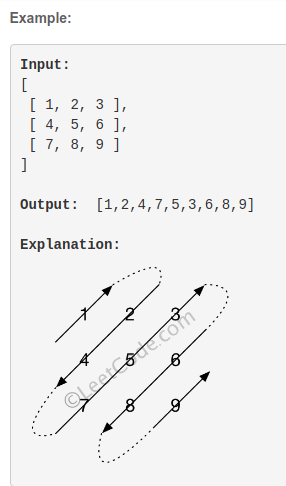
\includegraphics[width=150pt]{diagonal-traverse.png}\\
\figcaption{Diagonal Traverse}\label{fig:diagonal-traverse}
\end{center}

Note:
The total number of elements of the given matrix will not exceed 10,000.


\subsection{分析}
Nil

\subsection{代碼}
\begin{Code}
// LeetCode
// 時間複雜度O(),空間複雜度O()
class Solution {
public:
    vector<int> findDiagonalOrder(vector<vector<int>>& matrix) {
        int M = matrix.size();
        if (M == 0) return vector<int>();
        int N = matrix[0].size();
        if (N == 0) return vector<int>();

        vector<int> result; result.reserve(M + N);

        for (int d = 0; d < M + N - 1; d++) {
            int r = (d < N) ? 0 : d - N + 1;
            int c = (d < N) ? d : N - 1;

            vector<int> row;
            while (r < M && c > -1)
            {
                row.push_back(matrix[r][c]);
                r++;
                c--;
            }

            if (d % 2 == 0) reverse(row.begin(), row.end());
            result.insert(result.end(), row.begin(), row.end());
        }

        return result;
    }
};
\end{Code}

\subsection{代碼}
\begin{Code}
// LeetCode
// 時間複雜度O(),空間複雜度O()
class Solution {
public:
    vector<int> findDiagonalOrder(vector<vector<int>>& matrix) {
        if(matrix.empty()) return {};
        int m = matrix.size(), n = matrix[0].size();
        vector<int> res(m * n);
        for(int i = 0, r = 0, c = 0;i < m * n;i++) {
            res[i] = matrix[r][c];
            if((r + c) % 2 == 0) {
                if(c == n - 1) r++;
                else if(r == 0) c++;
                else r--, c++;
            } else {
                if(r == m - 1) c++;
                else if(c == 0) r++;
                else r++, c--;
            }
        }

        return res;
    }
};
\end{Code}
